\documentclass[conference]{IEEEtran}
\IEEEoverridecommandlockouts
% The preceding line is only needed to identify funding in the first footnote. If that is unneeded, please comment it out.
\usepackage{cite}
\usepackage{amsmath,amssymb,amsfonts}
\usepackage{algorithmic}
\usepackage{graphicx}
\graphicspath{ {images/} }
\usepackage{textcomp}
\usepackage{xcolor}
\def\BibTeX{{\rm B\kern-.05em{\sc i\kern-.025em b}\kern-.08em
    T\kern-.1667em\lower.7ex\hbox{E}\kern-.125emX}}
\begin{document}

\title{Utilization of Miners History Information to Prevent 51\% Attack on Proof-of-Work Blockchain\\
}

\author{
\IEEEauthorblockN{Xinle Yang, Yang Chen and David X. Chen}
\IEEEauthorblockA{\textit{MOAC Blockchain Tech Inc.} \\
Palo Alto, CA, USA \\
\{xinle.yang, yang.chen, david.chen\}@moac.io} 
}

\maketitle

\begin{abstract}
Proof-of-Work (PoW) is a popular protocol used in Blockchain systems to resolve double-spending problem. Major public Blockchains including Bitcoin, Ethereum, MOAC and many others are using PoW as mining protocol. When two or more miners generate branches of blocks that do not agree with each other, an accidental fork occurs. In this situation, under PoW protocol, the branch with largest total calculation difficulty will be selected to avoid double-spending problem. However, if an attacking node with calculation hash power greater than half of the total hash power, this attacking node can create a double-spending attack. This is attack is also called 51\% attack. With PoW protocol, the cost of creating a 51\% attack is quite inexpensive. We propose a technique to combine history information of miners with the total calculation difficulty to solve 51\% attack problem. Analysis indicates that with the new technique, the cost of a similar attack is increased by hundreds of times or more.
\end{abstract}

\begin{IEEEkeywords}
Blockchain, 51\% Attack, Mining, Double spending attack
\end{IEEEkeywords}

\section{Introduction}
Developed by Satoshi Nakamoto in 2009 \cite{b1}, Bitcoin is the first decentralized public ledger system. Since then, a number of similar blockchain-based cryptocurrencies have emerged. Blockchain is a distributed data processing protocol for retaining a public distributed ledger in a Peer-to-peer (P2P) network. Transaction data are recorded in blocks, and these blocks form a linked list (i.e., chain) of blocks. Each node in the network stores and maintains an entire copy of the ledger without requiring a central authority. In blockchain based cryptocurrencies, each block contains the hash value of the previous block, making it hard to manipulate the transactions within. Normally, a consensus protocol is used to guarantee the data integrity among the nodes of the blockchain P2P network. There are several different consensus protocols used in different types of blockchains \cite{b2}.

Proof-of-Work (PoW) is the most commonly used consensus protocol in blockchain based cryptocurrencies. Major blockchains such as Bitcoin and Ethereum are both using different variety of PoW protocol. In PoW protocol, each node is competing to find a nonce value to produce a hash that meets a certain criteria. The difficulty of calculating such a nonce value can be calculated based on the criteria of the hash value. When such a nonce value is found, a block is generated and broadcasted to the P2P network. Depends on different variety of protocol, peer nodes always accept the longest chain or the chain with the largest total difficulty repeatedly to continuously expand the blockchain. PoW utilizes this mechanism to determine which node has the right to seal a block. And, this process is also called mining.

In such a mechanism, a peer node with greater computing speed (or sometimes called hash rate power) can calculate nonce value faster than a peer node with less computing speed and thus has higher probability of getting the right to seal a new block. However, this mechanism has a drawback. A selfish node with hash rate power higher than those of the rest nodes combined can compromise the blockchain system by causing double spending and selfish mining, etc \cite{b3}\cite{b4}. This is commonly referred as a 51\% attack. Some studies have proposed ways to avoid such kind of attacks. Eyal and Sirer \cite{b5} in 2014 proposed a Two-Phase PoW (2P-PoW)solution preventing the formation of a mining pool with huge hash power. In this solution, the second phase PoW requires signature from the private key of the coinbase address. When the second PoW is sufficiently difficult, pool operators have to give out this private key to the pool miners in order to perform a calculation faster than all the peer nodes. Ruffing et al. \cite{b6} in 2015 proposed contracts to penalize attackers attempting a double-spending attack. Solat and Potop-Butucaru proposed ZeroBlock \cite{b7} in 2016. The mechanism in ZeroBlock requires a block to be accepted by its peers within certain time interval after the timestamp of the block. Otherwise, the block is expired. This mechanism prevent attacker node from selfish mining for a long period of time. J. Bae and H. Lim \cite{b8} in 2018 proposed a solution to randomly select a certain group of miners to have the right to mine the next block.

In this paper, we introduce a new solution by utilizing a historical weighted difficulty to determine the total chain difficulty. In such a modified algorithm, a branch of blockchain has a greater total historical weighted difficulty if the miners of such a branch have a higher coverage rate in previous blocks. We demonstrate that, in reality, such an algorithm can increase the money cost and the time cost of 51\% attack by a factor of at least two orders of magnitude.

\section{Historical weighted difficulty}
First, let us review the 51\% attack scheme. Assume current hashrate is $p$, attacker accumulate a greater hashrate power $p'$ with \text{$p' > p$}, and utilize this hashrate power to compute a hidden branch $B'$. Attacker performs double spending in two branches. Attacker then reveals hidden longer branch $B'$ and invalidate all transactions in original branch $B$. The cost to launch such a 51\% attack is,
\begin{equation}
Cost=(P*R)*f*t\label{eq}
\end{equation}
where $P$ is the token price, $R$ is the block reward, $f$ is the frequency of block generation speed, $t$ stands for the duration of the attack.
To many small blockchains, the cost to perform such an attack is only hundreds or thousands of US Dollars.

We propose a technique to calculate the total difficulty of a certain branch with the consideration of the miners addresses existence frequency in the previous blocks. We call this protocol HWD-PoW protocol. The assumption is that in an honest blockchain branch, miners of new blocks will most likely be the majority of the miners of the blocks previously mined. And, in a malicious blockchain branch, miners of new blocks will most likely only exists in a very limited ratio of miners in the blocks that are previously mined. Therefore, when mining history of miners are considered, one can easily distinguish an honest blockchain branch from a malicious one.

Under the proposed the mechanism, branch with miners of less representation in the previous blocks will earn less weight in the total difficulty calculation. Therefore, to perform a 51\% attack, the malicious miner have two choices: either to mine a much longer branch, or to build up miner representation in the previous blocks to build up the credibility.

Now, let us look at how Historical Weight Difficulty scheme works to defend the 51\% attack. 

(1) First, record each miner’s block generation frequency for history windows $W$:
\begin{equation}
r_i=\frac{(block\ mined\ by\ node\ i)}{(total\ block\ generated\ in\ window\ W)}\label{eq}
\end{equation}
where $\sum_{i=0}^{n}r_i = 1$

(2) Then, each block is then signed by miner's private key. By doing this, miners will not be able to counterfeit the miner address.

(3) When split happens, Historical Weighted Difficulty \text{$H\!W\!D$}  is calculated. For any miner $k$ in the branch $b$,
\begin{equation}
    H\!W\!D_b = \sum_{k=0}^{l}r_k\label{eq}
\end{equation}

(4) Peer nodes compare two different \text{$H\!W\!D$}'s from two branches. And, the branch with greater \text{$H\!W\!D$} will be selected.

Scenario 1: If attacker just brings in temporary new hashrate power, even if the hidden branch is longer in difficulty, but the miner of the new branch is relatively new to the system, so the $r_i$ of the blocks is very low. The corresponding \text{$H\!W\!D$} will be very little compared to the original branch. No peer node in the original branch will switch to the attacker branch. 

Scenario 2: In order to gain historical weight of the miner, the attacker can mine in the original branch for a while, make itself included in the history. Therefore, when it switches to hidden branch, it’s \text{H\!W\!D} will be greater. 

Suppose $p'$ is the attacker miners' hashrate, $p0$ is the honest miners' hashrate.

\begin{figure}[htbp]
\centerline{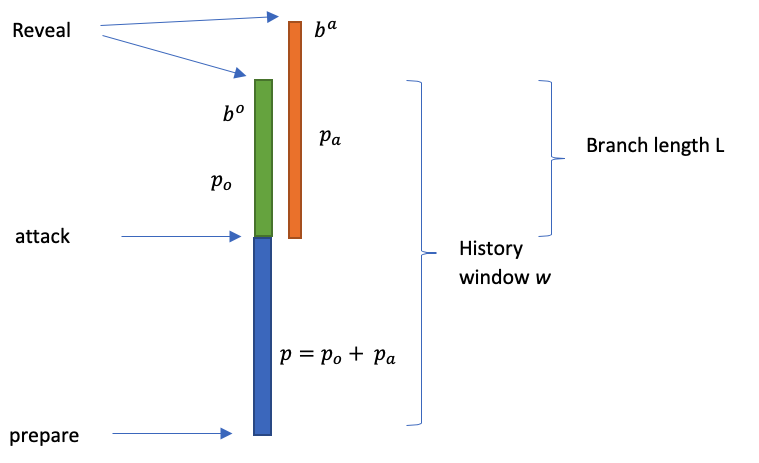
\includegraphics[width=3in]{figure.png}}
\caption{Attacker tries to attack branch $b$ with branch $b'$.}
\label{fig}
\end{figure}

Let's look at the cost of this setup. Attacker needs to spend hashrate $p'$ in the original branch for a time duration $t'$. The optimum spending of $p'$ is to mine for $w/2$ period and then switch $p'$ to hidden branch. 

At attack time point, assume
\begin{equation}
    H\!W\!D_b= \sum_{k=0}^{l}r'_k=\frac{1}{2} + \delta\label{eq}
\end{equation}
In order for attack to be successful, At the reveal time, \text{$H\!W\!D$} of the malicious branch is,
\begin{equation}
    H\!W\!D_b= (\frac{1}{2} + \delta) * \frac{w-l}{w}\label{eq}
\end{equation}
\text{$H\!W\!D$} of the original branch is,
\begin{equation}
    H\!W\!D_0 = \sum_{k=0}^{l} r_{k}^{0} =  \frac{1}{2} - \delta\label{eq}
\end{equation}
Therefore, the following condition must satisfy,
\begin{equation}
    (\frac{1}{2} + \delta) * \frac{w-l}{w} > \frac{1}{2}-\delta\label{eq}
\end{equation}
where
\begin{equation}
\delta>\frac{l}{4w-2l}\label{eq}
\end{equation}
To summarize, attacker needs to prepare for $(w-l)$ duration with hashrate $1/2+l/(4w-2l)$.

For a typical attack, $l$ needs to be around 100-500 block to allow token withdrawn from token exchange. We need to have $w > 1 month$ to increase the history weight to attack. With $w = 100,000$, the robustness is increased by over 100 time. 

In the above scenarios, although we cannot totally avoid 51\% attach, but we increased the money cost and time cost of such an attack to at least two orders of magnitude.

Also, this mechanism can be more secured if we introduce another condition such as by requiring the new branch with certain amount of miner overlap with the old branch. Under such a condition, in order for a branch switch to happen, one needs to satisfy not only the \text{$H\!W\!D$} condition,
\begin{equation}
    H\!W\!D_b>H\!W\!D_0\label{eq}
\end{equation} 
but also, the overlap of old miners and new miners need to be greater than $s$,
\begin{equation}
    \{r_i\}\bigcap\{r_k\}>s\label{eq}
\end{equation}
Meaning, the system discourages sudden hash power switch from one set of miners to another distinct set of miners.

With such an enhanced requirement, if $s=0.25$, attacker needs to have two times of the current hashrate with time duration $w$. Which means attacker needs to keep some hashrate in the original branch, and twice more in the malicious branch to compensate the effect. Therefore, by introducing such a requirement, we double the time cost and tripled the money cost to perform an attack to the original Historical Weighted Difficulty algorithm.

\section{Real data statistics from Ethereum}

We picked a well-known PoW blockchain platform Ethereum. We investigated block data of 2,000,000, 4,000,000, 6,000,000 and following 360 blocks for each from Ethereum Mainnet.

\begin{table}[htbp]
\caption{Ethereum block miners from 2,000,001 to 2,000,360}
\begin{center}
\begin{tabular}{lclclcl}
\hline
Miner                                      & Weight   & Amount & Weight\_in\_2M \\
\hline
0x1654......d5de & 0.002778 & 1      & 0.001272       \\
0x186a......b0f2 & 0.002778 & 1      & 0.000001       \\
0x1a06......58f1 & 0.030556 & 11     & 0.004212       \\
0x2a65......8226 & 0.272222 & 98     & 0.239315       \\
0x2cb7......6402 & 0.002778 & 1      & 0.000004       \\
0x30b6......4e6d & 0.002778 & 1      & 0.002430       \\
0x40ce......f821 & 0.002778 & 1      & 0.000954       \\
0x4bb9......1b01 & 0.063889 & 23     & 0.057752       \\
0x52bc......e3b5 & 0.038889 & 14     & 0.147223       \\
0x5979......e584 & 0.002778 & 1      & 0.000116       \\
0x61c8......0bd9 & 0.177778 & 64     & 0.049251       \\
0x6879......01da & 0.025000 & 9      & 0.023600       \\
0x6caf......a46d & 0.002778 & 1      & 0.001050       \\
0x7a14......0b95 & 0.002778 & 1      & 0.001233       \\
0x9148......a49d & 0.002778 & 1      & 0.000021       \\
0x94ce......a2f7 & 0.002778 & 1      & 0.000944       \\
0x9558......7211 & 0.002778 & 1      & 0.011990       \\
0xa027......e88f & 0.005556 & 2      & 0.012287       \\
0xa42a......e84e & 0.055556 & 20     & 0.001293       \\
0xadd8......db02 & 0.002778 & 1      & 0.000039       \\
0xbcdf......41d1 & 0.163889 & 59     & 0.023924       \\
0xd138......a31c & 0.005556 & 2      & 0.000053       \\
0xd3d0......ee9d & 0.002778 & 1      & 0.001598       \\
0xdc3f......e455 & 0.002778 & 1      & 0.000340       \\
0xea67......8ec8 & 0.116667 & 42     & 0.036458       \\
0xf3b9......c2fb & 0.005556 & 2      & 0.008294      \\
\hline
\multicolumn{4}{l}{$^{\mathrm{a}}$Toal miners' weight from previous 2 million blocks is 62.57\%.}
\end{tabular}
\end{center}
\end{table}

\begin{table}[htbp]
\caption{Ethereum block miners from 4,000,001 to 4,000,360}
\begin{center}
\begin{tabular}{lclclcl}
\hline
Miner                                      & Weight   & Amount & Weight\_in\_4M \\
\hline
0x1e99......0341 & 0.138889 & 50     & 0.039864       \\
0x2a65......8226 & 0.072222 & 26     & 0.203597       \\
0x4bb9......1b01 & 0.016667 & 6      & 0.058306       \\
0x52bc......e3b5 & 0.075000 & 27     & 0.096536       \\
0x73b8......7fea & 0.005556 & 2      & 0.003767       \\
0x829b......a830 & 0.283333 & 102    & 0.006120       \\
0x8727......87a5 & 0.005556 & 2      & 0.000166       \\
0x9435......7805 & 0.008333 & 3      & 0.001669       \\
0x9633......a11c & 0.008333 & 3      & 0.002592       \\
0xa027......e88f & 0.002778 & 1      & 0.006821       \\
0xa42a......e84e & 0.005556 & 2      & 0.017388       \\
0xa4aaf......7f0d & 0.005556 & 2      & 0.001638       \\
0xa9a9......51fc & 0.002778 & 1      & 0.000456       \\
0xb293......0347 & 0.086111 & 31     & 0.016308       \\
0xc0ea......2949 & 0.033333 & 12     & 0.036065       \\
0xea67......8ec8 & 0.236111 & 85     & 0.102737       \\
0xf3b9......c2fb & 0.013889 & 5      & 0.011940      \\
\hline
\multicolumn{4}{l}{$^{\mathrm{a}}$Toal miners' weight from previous 4 million blocks is 65.60\%.}
\end{tabular}
\end{center}
\end{table}

\begin{table}[htbp]
\caption{Ethereum block miners from 6,000,001 to 6,000,360}
\begin{center}
\begin{tabular}{lclclcl}
\hline
Miner                                      & Weight   & Amount & Weight\_in\_6M \\
\hline
0x0019......99e8 & 0.002778 & 1      & 0.000262   \\
0x1ca4......be1a & 0.019444 & 7      & 0.000301   \\
0x2a65......8226 & 0.027778 & 10     & 0.147516   \\
0x35f6......738d & 0.005556 & 2      & 0.000108   \\
0x4a07......a82b & 0.005556 & 2      & 0.000993   \\
0x4bb9......1b01 & 0.002778 & 1      & 0.044112   \\
0x52bc......e3b5 & 0.116667 & 42     & 0.106200   \\
0x52e4......f13c & 0.013889 & 5      & 0.002402   \\
0x5a0b......9c4c & 0.133333 & 48     & 0.036217   \\
0x6a7a......9b1f & 0.008333 & 3      & 0.002958   \\
0x70ae......e21d & 0.008333 & 3      & 0.000786   \\
0x829b......a830 & 0.127778 & 46     & 0.074208   \\
0x914d......1dcd & 0.002778 & 1      & 0.000056   \\
0x92e3......b549 & 0.002778 & 1      & 0.000274   \\
0x9435......7805 & 0.002778 & 1      & 0.003470   \\
0xb293......0347 & 0.105556 & 38     & 0.043726   \\
0xb75d......22f5 & 0.011111 & 4      & 0.001900   \\
0xb8f8......5453 & 0.002778 & 1      & 0.000222   \\
0xcc16......e610 & 0.002778 & 1      & 0.000742   \\
0xd100......4fce & 0.002778 & 1      & 0.000157   \\
0xd380......636d & 0.002778 & 1      & 0.000000   \\
0xd438......1807 & 0.011111 & 4      & 0.000198   \\
0xd958......4012 & 0.013889 & 5      & 0.000088   \\
0xd9cf......06e3 & 0.002778 & 1      & 0.000036   \\
0xe4bd......0649 & 0.005556 & 2      & 0.001237   \\
0xea67......8ec8 & 0.322222 & 116    & 0.154956   \\
0xf3b9......c2fb & 0.036111 & 13     & 0.015957  \\
\hline
\multicolumn{4}{l}{$^{\mathrm{a}}$Total miners' weight from previous 6 million blocks is 63.91\%.}
\end{tabular}
\end{center}
\end{table}

From the above data, we can see that the total miner appearance rate is $62.57\%$, $65.60\%$ and $63.91\%$. All of which are around over $60\%$. The cost of attacking such a chain under regular Ethereum PoW protocol is $361$ Ether. Under HWD-PoW protocol, if attacker appeared in $1\%$ of pervious blocks, total cost of performing an attack will be calculated as follow,
\begin{equation}
    Cost = r_i * W + \frac{360 * 60\%}{r_i}\label{eq}
\end{equation}
The actual cost of the three scenarios under HWD-PoW protocol are 41,601 Ethers, 61,601 Ethers and 81,601 Ethers respectively. Comparing with the original PoW protocol, the cost increases are 114, 170 and 225 times respectively.

\section{Conclusion}

In this paper, we have proposed an approach to increase the cost of a successful double-spending attack on Proof-of-Work types of Blockchain protocols. The proposed approach reads the appearance rate of miners in history blocks and calculates the total Historical Weighted Difficulty. We demonstrated in three real Ethereum Mainnet scenarios, the cost of attack is increased by more than 100 times.

\section*{Acknowledgment}

This work was supported by MOAC foundation and MOAC Blockchain Tech Inc.

\begin{thebibliography}{00}

\bibitem{b1} S. Nakamoto,``Bitcoin: A peer-to-peer electronic cash system," 2008.
\bibitem{b2} Z. Zheng, S. Xie, H. Dai, X. Chen, and H. Wang, ``Blockchain challenges
and opportunities: A survey," Internat. J. Web Grid Serv., 2016.
\bibitem{b3}M. Conti, S. Kumar E, C. Lal, and S. Ruj, ``A survey on security and privacy issues of Bitcoin," arXiv preprint arXiv:1706.00916, 2017.
\bibitem{b4} Eyal, I. and Sirer, E.G. (2014) ``Majority is not enough: Bitcoin mining is vulnerable", Proceedings
of International Conference on Financial Cryptography and Data Security, Berlin, Heidelberg,
pp.436–454.
\bibitem{b5} I. Eyal and E. G. Sirer, ``How to disincentivize large Bitcoin mining pools," 2014.
\bibitem{b6} T. Ruffing et al., “Liar, liar, coins on fire!: Penalizing equivocation by loss of Bitcoins," ACM Conf. Comput. Commun. Secur., Oct. 2015.
\bibitem{b7} S. Solat and M. Potop-Butucaru,``ZeroBlock: Preventing selfish mining in Bitcoin," arXiv preprint arXiv:1605.02435, 2016.
\bibitem{b8} J. Bae and H. Lim, ``Random Mining Group Selection to Prevent 51\% Attacks on Bitcoin," 2018 48th Annual IEEE/IFIP International Conference on Dependable Systems and Networks Workshops (DSN-W), Luxembourg City, 2018, pp. 81-82.
doi: 10.1109/DSN-W.2018.00040
\end{thebibliography}
\vspace{12pt}
\color{red}

\end{document}
